%  Architecture.tex
%  Document created by seblovett on seblovett-Ubuntu
%  Date created: Thu 17 Apr 2014 14:55:41 BST
%  <+Last Edited: Sun 11 May 2014 10:13:31 BST by seblovett on seblovett-Ubuntu +>


\chapter{Architecture}

\review{Architecture}

%Design of the datapath architecture.

%Refer to the research done and how this influenced the design

The architecture for the processor was initially designed on a MIPS datapath.
Support was then added to allow the ARM Thumb architecture (see Chapter~\ref{ch:is}) to be executed on the datapath.
Extra aspects to the datapath were then added based on the research done. 
The full datapath diagram is seen in Figure~\ref{fig:architecture}.

A Link Register is used to improve the speed when calling leaf functions.
The original design also included a dedicated Stack Pointer, however this was later removed during the project.
The convention of using Register 7 as the Stack Pointer was instead used. 
Both of these aspects were added from the recomendations from the research report on subroutines.

The processor supports four flags: carry, overflow, negative and zero. 
It is a two operand register-register design.
There are eight general purpose registers with no dummy register. 

The datapath was also modified during the project to allow for interrupt support.
These changes included a input to the Program Counter to jump to a specific location, reading and writing of the status register from and to the system bus, and input of the Program Counter directly from the system bus. 

\inote{HSL: I don't know how in depth we should go here as we talk about everything later on}

\begin{figure}
%%\missingfigure{Architecture diagram}
%\hspace*{-1in}
\vspace*{-1.5in}
\makebox[\linewidth]{
\centerline{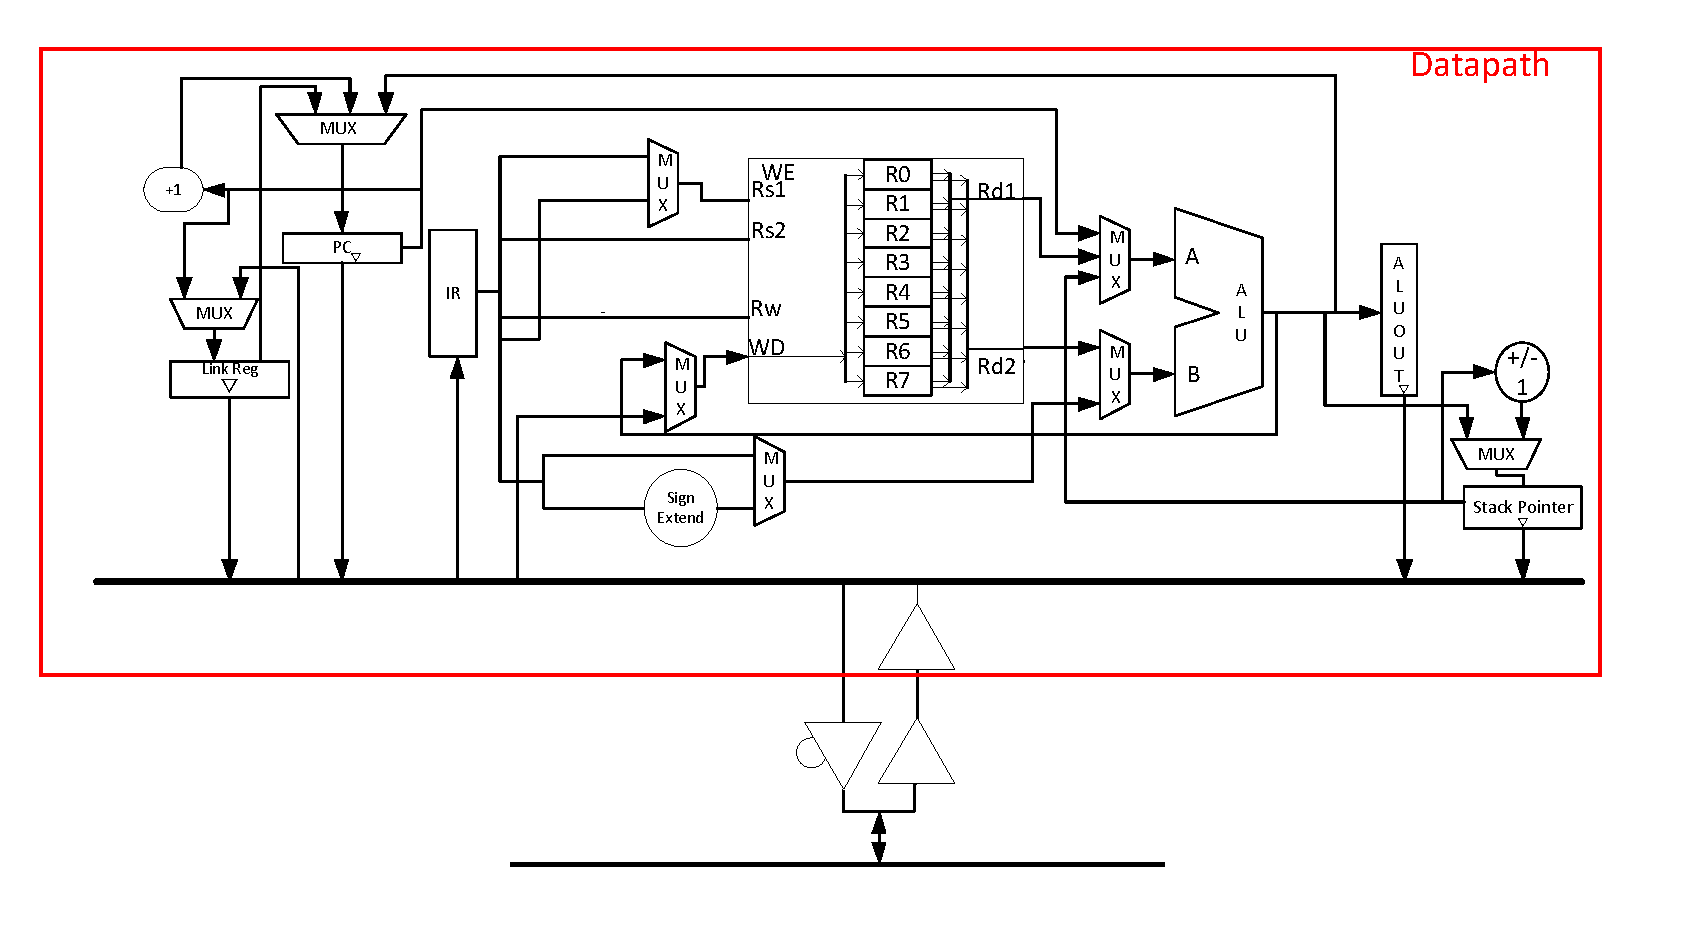
\includegraphics[angle=270,width=\textwidth-2.5cm]{../../Design/RandD/idea1.pdf}}
}
\caption{The Architecture diagram of the processor.}
\label{fig:architecture}
\end{figure}

